\subsection{Monarch Initiative: Mendelian-disease causality and phenotypic breadth}
\label{sec:monarch}
The GWAS audit (Section~\ref{sec:gwas}) tested common-variant germline
associations of the panel; here we test the complementary rare/Mendelian
axis. We queried the Monarch Initiative knowledge graph v3 (aggregating
OMIM, Orphanet, and HPO annotations) for causal and correlated
gene--disease associations and HPO phenotype annotations of all @NGENES@
study genes (@NRES@ resolved to HGNC identifiers; the remainder recorded as
unresolved).

\paragraph{Calibration gate.} Pre-registered gates PASSED: (G1) @NRES@/@NGENES@
genes resolved (threshold 180); (G2) the CD19 sentinel carries at least one
causal gene--disease association (observed @CDTWO@; OMIM common variable
immunodeficiency 3); (G3) CD19 carries at least ten HPO phenotype
annotations (observed @CDTHREE@). Gate thresholds were calibrated on a
recorded connectivity probe of the live API before the full fetch.

\paragraph{Causality gated versus background.} Genes carrying at least one
causal (Mendelian) disease association: @H1G@/@H1GN@ gated versus @H1B@/@H1BN@
background (Fisher odds ratio @H1OR@, $p=@H1P@$). Correlated (non-causal)
disease associations: @H3G@/@H3GN@ versus @H3B@/@H3BN@ (odds ratio @H3OR@,
$p=@H3P@$). Median HPO phenotypic breadth @H2G@ versus @H2B@
(Mann--Whitney $p=@H2P@$). Restricting causal associations to disease labels
matching cancer terms: @H4G@/@H4GN@ gated versus @H4B@/@H4BN@ ($p=@H4P@$).
@VERDICT@

\paragraph{AND-gate antigens.} @ANTIGENBLOCK@

\begin{figure}[t]
\centering
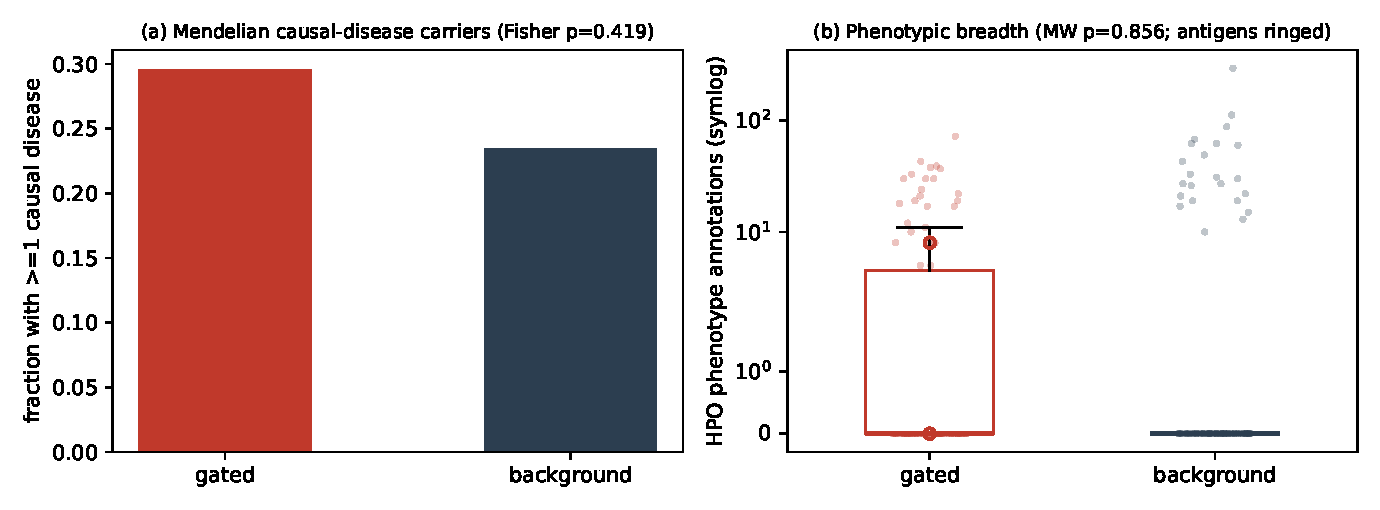
\includegraphics[width=\linewidth]{monarch_fig.pdf}
\caption{Monarch Mendelian-disease and phenotype audit. (a) Fraction of
genes carrying at least one causal gene--disease association. (b) HPO
phenotypic breadth per gene (symlog axis), with the seven AND-gate
antigens ringed.}
\label{fig:monarch}
\end{figure}
